\documentclass{sig-alternate}
\pdfpagewidth=8.5in
\pdfpageheight=11in
\special{papersize=8.5in,11in}

%%%%%%%%%%%%%%%%%%%%%%%%%%%%%%%%%%%%%%%%%%%%%%%%%%%%%%
% Packages
\usepackage{bm}
\usepackage{graphicx}
\usepackage{tabularx}
\usepackage[dvipsnames]{xcolor}
\usepackage{xspace}
\usepackage{float}
\usepackage{rotating}
\usepackage{xstring} % for string operations
\usepackage{wasysym} % Table legend with symbols input from post-processing
\usepackage{MnSymbol} % Table legend with symbols input from post-processing
%\usepackage[hidelinks]{hyperref} % make COCO papers clickable

%%%%%%%%%%%%%%%%%%%%%%%%%%%%%%%%%%%%%%%%%%%%%%%%%%%%%%
% Definitions

% Algorithm names as they appear in the tables, uncomment if necessary
%\newcommand{\algAtables}{\algaperfprof}  % first argument in the post-processing
%\newcommand{\algBtables}{\algbperfprof}  % first argument in the post-processing
%\newcommand{\algCtables}{\algcperfprof}  % first argument in the post-processing
%\newcommand{\algDtables}{\algdperfprof}  % second argument in the post-processing
%\newcommand{\algEtables}{\algeperfprof}  % second argument in the post-processing
% location of pictures files
\newcommand{\bbobdatapath}{comparison/}
\input{\bbobdatapath bbob_pproc_commands.tex}
\graphicspath{{\bbobdatapath}}
\newcommand{\algname}{IBEA}

%%%%%%%%%%%%%%%%%%%%%%%%%%%%%%%%%%%%%%%%%%%%%%%%%%%%%%
% pre-defined commands
\newcommand{\DIM}{\ensuremath{\mathrm{DIM}}}
\newcommand{\aRT}{\ensuremath{\mathrm{aRT}}}
\newcommand{\FEvals}{\ensuremath{\mathrm{FEvals}}}
\newcommand{\nruns}{\ensuremath{\mathrm{Nruns}}}
\newcommand{\Df}{\ensuremath{\Delta f}}
\newcommand{\DI}{\ensuremath{\Delta I}}
\newcommand{\nbFEs}{\ensuremath{\mathrm{\#FEs}}}
\newcommand{\fopt}{\ensuremath{f_\mathrm{opt}}}
\newcommand{\ftarget}{\ensuremath{f_\mathrm{t}}}
\newcommand{\Itarget}{\ensuremath{I_\mathrm{target}}}
\newcommand{\CrE}{\ensuremath{\mathrm{CrE}}}
\newcommand{\change}[1]{{\color{red} #1}}
\newcommand{\bbobbiobj}{{\ttfamily bbob-biobj}\xspace}
\newcommand{\hvref}{I^{\mathrm{ref}}}
\newcommand{\TODO}[1]{{\color{red} TODO: #1}}

    \renewcommand{\topfraction}{1}	% max fraction of floats at top
    \renewcommand{\bottomfraction}{1} % max fraction of floats at bottom
    %   Parameters for TEXT pages (not float pages):
    \setcounter{topnumber}{3}
    \setcounter{bottomnumber}{3}
    \setcounter{totalnumber}{3}     % 2 may work better
    \setcounter{dbltopnumber}{4}    % for 2-column pages
    \renewcommand{\dbltopfraction}{1}	% fit big float above 2-col. text
    \renewcommand{\textfraction}{0.0}	% allow minimal text w. figs
    %   Parameters for FLOAT pages (not text pages):
    \renewcommand{\floatpagefraction}{0.80}	% require fuller float pages
    % N.B.: floatpagefraction MUST be less than topfraction !!
    \renewcommand{\dblfloatpagefraction}{0.7}	% require fuller float pages

%%%%%%%%%%%%%%%%%%%%%%%%%%%%%%%%%%%%%%%%%%%%%%%%%%%%%%

\begin{document}

\IfFileExists{\bbobdatapath ppfig2_f001.pdf}{2 algorithms currently not supported}{}

\title{Benchmarking of the Indicator-based evolution algorithm using the Bi-Objective BBOB Test Suite
% \titlenote{If needed}
}
\subtitle{Final report
\titlenote{Submission deadline: October 21st.}}

\numberofauthors{5}
\author{
\alignauthor 
Daro Heng
\alignauthor
Karim Kouki
\alignauthor
Ahmed Mazari
\and
\alignauthor 
Mihaela Sorostinean
\alignauthor 
Aris Tritas
}

\maketitle
\begin{abstract}
The objective of this project was to study, implement and benchmark the Indicator Based Evolutionary Algorithm \\ (IBEA) using  the Comparing Continuous Optimizer (COCO) platform. Firstly we provide a brief overview of the algorithm. Secondly, we describe our implementation and experimental setup. Finally, we discuss the obtained results and compare them to both baseline approaches and related work.
\end{abstract}

\section{Setting}
In the context of a multi-objective optimization, the main goal is to find a good approximation of the set of Pareto-optimal solutions.
An evolutionary algorithm is an exploration strategy of the domain space $\mathbb{R}^n$ which seeks optimal solution vectors defined in the objective space $\mathbb{R}^k$ (here $k=2$).

The performance measure used by IBEA for determining the relative quality of two solution sets in the objective space is a binary indicator function $I: \Omega \times \Omega \rightarrow \mathbb{R}$. 
In terms of two decision vectors $\bm{x}^1$ and $\bm{x}^2$,  the \textit{domination} relation is defined as : $\bm{x}^1 \succ \bm{x}^2 \leftrightarrow ( f_i(\bm{x}^1) \leq f_i(\bm{x}^2) \; \forall i \in \{1, ..., n\} \;\text{and}\; f_j(\bm{x}^1) < f_j(\bm{x}^2)$ for at least one objective$)$. 
The epsilon indicator is compliant with this dominance relationship and defined for pairwise comparisons as: $$I_{\epsilon^+} (\{\bm{x}^1\}, \{\bm{x}^2\}) = \min_\epsilon f_i(\bm{x}^1) - \epsilon \leq f_i(\bm{x}^2) \; \forall i \in \{1, ..., n\}$$. 
It reduces the minimum distance to improve on the Pareto set approximation to a single scalar. 
Intuitively, this may incur a  loss of information with respect to each dimension of the multi-objective optimization. 
Indeed, we are required to choose the minimum distance of improvement across all objectives. However, the fact that we choose to \emph{conservatively} improve on the fitness estimate means that we may miss on potential improvement on one or more objectives.

The fitness value is defined in the sequel as a measure of the usefulness of each individual with regards to the optimization goal. As such, the algorithm tries to maximize it.
$$ F(\bm{x}^1) = \sum_{\bm{x}^2 \in P \setminus \{\bm{x}^1\}} - \exp{\frac{I(\{\bm{x}^1\}, \{\bm{x}^2\})}{\kappa}}$$ where $P$ is the population set, and $\bm{x} \in \mathbb{R}^n$. The fitness function of an approximation set is defined as a \emph{dominance preserving relation}.

The domain space typically has axes with different scales. Therefore, Adaptive-IBEA scales the objective function values as well as the range of values taken by the indicator function. This scheme decreases the need parameter tuning in face of problem and indicator function diversity.

\section{Implementation}
The input of the algorithm is the size of the population ($\alpha$), a maximum number of generations (corresponding to the budget) set as termination criterion and a fitness scaling factor ($\kappa$). The output of the algorithm is an approximation of the Pareto-set.
\begin{enumerate}
\item \textbf{Initialization:} randomly generate an initial population P of the given size and set generation counter to 0.
\item \textbf{Fitness assignment:} computate and assign a fitness value to each individual in P.

\item \textbf{Environmental selection:} detect and remove individuals which have the smallest fitness values from the population until the current size of the population P does not exceed $\alpha$. Update the fitness values for all remaining individuals.

\item \textbf{Termination:} after the environmental selection is performed, the termination criterion of the algorithm is checked; if the maximum number of generations is reached or another termination criterion is met, the algorithm returns the set of decision vectors A.

\item \textbf{Mating Selection:} consists in creating as temporary mating pool P' which is filled with individuals from P by performing binary tournament selection with replacement on P.

\item \textbf{Variation:} finally the variation step consists applying recombination and mutation operators to the previously created mating pool. In this case, the operator SBX-20 was chosen for the recombination part, while a polynomial distribution was used for the mutation part.  The offspring resulted after applying these operators is added to P, while also incrementing the generation counter. The algorithm is then performed again from step 2, until a termination criterion is met.

\end{enumerate}
As far as the implementation in Python is concerned we chose to represent the population in a compact data structure and did all numerical computation with NumPy. The steps of the algorithm were inlined in a single optimization function, except for the recombination and mutation operators which were implemented in separate functions to achieve modularity during testing.

Python dictionary, grid search

\section{Experiments}
\subsection{La galere}
 For the first part of the project our milestone was to have a working version of the algorithm, and potentially reasonable results on at least some groups of functions.
 
Without further changes to the original strategy, our algorithm does not seem to reach the optimal Pareto set of solution vectors. We tried applying recombination and mutation with high and low probabilities respectively, following the literature. This did not yield improved results, which leads us to think that either our implementation lacks robustness, or has a subtle bug.

We intended to:
\begin{enumerate}
\item Experiment with self-adaptive strategies for the mutation step, and 
\item Implement Self-Adaptive SBX which seeks an optimal index for the approximation distribution used
\end{enumerate}
\subsection{Setup}
The proposed implementation of the IBEA algorithm was tested with the collection of benchmark problems comprised in the COCO platform. We performed several experiments with various combinations of parameters in order to evaluate the influence of specific parameters on the results for different categories of benchmark problems. Therefore we varied the following parameters:
\begin{itemize}
\item The budget - various values between 300, 500, 750, 850, 1000
\item Population size - varied between 50, 60, 80, 100, 200
\item Number of offspring - 20, 30 or 40
\item Mutation probability - 0.7, 0.8, 0.9, 1.0
\item Recombination probability - or probability of crossover for the recombination step - 0.4, 0.6, 0.8, 0.9, 1.0
\item Variance - 1.3 , 2.5, 5, 10, 15
\item Offspring : - 20, 30, 35, 40
\item Dimension : 2, 5, 10, 20, 40
\item Max iterations: $10^6$, $10^9$
\item Distribution index for the SBX operator: 2, 5 or 20 (the value suggested by the authors)
\item Operators : Isotropic, Derandomized
\end{itemize}

Since the number of variable parameters was considerable, carrying experiments with all combinations between them was impossible, so we selected a limited number of combinations which we considered might give significant results. The sets of parameters that we used in our experiments are illustrated in table 1.  
Running a bi-objective algorithm in a laptop is not an easy task. It's both time and RAM consuming.  The execution takes from 5 to 23 hours to finish with a budget of 1000. The timing experiment  is intrinsically associated with the size of the population and the dimension. 
For that reason, we tried only one configuration for 40 dimensions that took almost 48h  with a moderate budget of 300.  
In order to try several parameterizations of the algorithm we  were obliged to make non stopping running of the algorithm on different machine with different parameter in order to evaluate how  the algorithm performs under different parameterizations. We conclude from this empirical study that a high variance and low variance impacts negatively the performance of the algorithm. The trick is to find a trade-off between the size of population, variance and the recombination values.

\subsection{Recombination}

The operator we used were intermediate weighting, discrete recombination  and finally, the Simulated Binary Crossover \cite{deb1994simulated}. However, results using these operators were not encouraging. The reason for that may be a rather naive exploration of the search space.

In this case, the Simulated Binary Operator was chosen for the recombination part.
\subsection{Variation}

For the mutation step, we simply added isotropic Gaussian noise with fixed variance to the produced offspring. However, it is well known that fixing variance does not speed up search optimally.
a polynomial distribution was used for the mutation part.  
%%%%%%%%%%%%%%%%%%%%%%%%%%%%%%%%%%%%%%%%%%%%%%%%%%%%%%%%%%%%%%%%%%%%%%%%%%%%%%%
\section{CPU Timing}
%%%%%%%%%%%%%%%%%%%%%%%%%%%%%%%%%%%%%%%%%%%%%%%%%%%%%%%%%%%%%%%%%%%%%%%%%%%%%%%
% note that the following text is just a proposal and can/should be changed to your needs:
In order to evaluate the CPU timing of the algorithm, we have run the \algname with restarts on the entire bbob-biobj test suite \cite{biobj2016func} for $2 D$ function evaluations. The Python code was run on a Intel(R) Core(TM) i5-2400S CPU @ 2.50GHz with 4 processors and 8 cores. The time per function evaluation for dimensions 2, 3, 5, 10, 20 equals $1.7e{-3}$, $1.9e{-3}$, $2.0e{-3}$, $2.2e{-3}$, $2.4e{-3}$ seconds respectively.  


%%%%%%%%%%%%%%%%%%%%%%%%%%%%%%%%%%%%%%%%%%%%%%%%%%%%%%%%%%%%%%%%%%%%%%%%%%%%%%%
\section{Results}
%%%%%%%%%%%%%%%%%%%%%%%%%%%%%%%%%%%%%%%%%%%%%%%%%%%%%%%%%%%%%%%%%%%%%%%%%%%%%%%

Results of \algname\ from experiments according to \cite{hansen2016exp} and \cite{brockhoff2016biobjective} on the benchmark
functions given in \cite{biobj2016func} are presented in
Figures~\ref{fig:ECDFsingleOne}, \ref{fig:ECDFsingleTwo}, \ref{fig:ECDFsingleThree}, and \ref{fig:ECDFsGroups}, and in
Table~\ref{tab:aRTs}. The experiments were performed with COCO \cite{hansen2016cocoplat}, version 1.0.1, the plots were produced with version 1.0.4.
\subsection{Comparison of isotropic and derandomized mutation operators}
Derandomized mutation performs better on the following functions: (initial variance is 5, mutation prob is 0.8, crossover is  SBX-5 and Pr(0.8))
\begin{itemize}
\item Rosenbrock function 28.
\item Function 23
\item Much better on functions 26 \& 34
\item Function 2
\end{itemize}
By using $\alpha = 80$ and offsprings 30, better results were obtained for the following functions:
\begin{itemize}
\item function 13 (as well as function 12)
\item function 16
\item function 19
\item 2-moderate 4-multi-modal:  no good results in function group overall except for a slight improvement with this configuration on function 25
\end{itemize}

Function 15: Isotropic : Variance of 5 better than variance of 10, 
			 Derandomized: Smaller population as good as isotropic with small variance
			 
\subsubsection*{1-separable 2-moderate (3d)}: 
low mutation (0.1) is better for functions 12 and 13 and/or high recombination probability (>=0.8) is bad (why?)

smaller initial variance (3) is better for f13

\subsubsection*{1-separable 4-multi-modal} : high variance (10) is bad

\subsubsection*{1-separable 5-weakly-structured}
function 18: High recombination probability (0.7-0.9)
			  High mutation probability (around 0.7-0.8)  (along with isotropic pop 100)
			  High variance is bad

\subsubsection*{2-moderate 2-moderate}
Variance is a critical factor. 
Mutation with probability 1 without adaptation of the variance gives worse results.
Function 20 gives good results with mut0.3 in 5d - best mut0.3 recomb0.7 
28-2d as good for pop100 offs20 mut0.1 recomb0.7 var5.0 as for pop100 offs20 mut0.8 recomb0.6

\subsubsection*{2-moderate 5-weakly-structured}
Better results with low mutation probability (0.1-0.3)
Function 33: good results with relatively higher variance. Improved for a smaller population and moderate variance
26, 33: best with mut0.8 recomb0.6

\subsubsection*{3-ill-conditioned 3-ill-conditioned} 
variance is not the determinating factor. Isotropic a little worse.

Function 42: Derandomized and/or Higher population are better than pop=60

\subsubsection*{3-ill-conditioned 5-weakly-structured} 
High variance doesn't hurt w.r.t a smaller one. - 
Can't say much though because the problems are unstructured and hard)
f44-5d: mut0.8 recomb0.7 var5.0derandomized sbx2

\subsubsection*{4-multi-modal 4-multi-modal} 
Derandomized improves a tiny bit on isotropic.
\subsubsection*{4-multi-modal 5-weakly-structured}
 Function 48: high variance does not perform worse, on other functions of  derandomized is better
								    
Functions 54, 55: Can't say much. Derandomized/Smaller variance better.

Cases in which low mutation probability works:
2-moderate 5-weakly-structured: best is 0.3
3-ill-conditioned 5-weakly-structured: function 44 has good results

For 5-d space:
Function 53 performs very well with pop80, mut0.8, recombination1.0, derandomized
On the other hand it performs well with low mutation probability (0.1-0.3) on 3d
Find solutions really quick with var 3.

\subsection{aRT}
We observe with no surprise that our algorithm has a runtime of $1e{-3}$ iff the variance is adapted. gets to 10-3 on f12

We also observe that using a better indicator tends to find targets much faster.

%%%%%%%%%%%%%%%%%%%%%%%%%%%%%%%%%%%%%%%%%%%%%%%%%%%%%%%%%%%%%%%%%%%%%%%%%%%%%%%
\section{Results}
%%%%%%%%%%%%%%%%%%%%%%%%%%%%%%%%%%%%%%%%%%%%%%%%%%%%%%%%%%%%%%%%%%%%%%%%%%%%%%%

Results from experiments according to \cite{hansen2016exp},
\cite{hansen2016perfass} and \cite{biobj2016perfass} on the benchmark
functions given in \cite{biobj2016func} are presented in
Figures~\ref{fig:ECDFsingleOne}, \ref{fig:ECDFsingleTwo}, \ref{fig:ECDFsGroupsFive} and
\ref{fig:ECDFsGroupsTwenty} and in Tables~\ref{tab:aRTs5} and~\ref{tab:aRTs20}.
The experiments were performed with COCO \cite{hansen2016cocoplat}, version
\change{1.0.1}, the plots were produced with version \change{1.1.1}.

The \textbf{average runtime (aRT)}, used in the %figures and
tables,
depends on a given quality indicator value, $\Itarget=\hvref+\DI$, and is
computed over all relevant trials as the number of function
evaluations executed during each trial while the best indicator value
did not reach \Itarget, summed over all trials and divided by the
number of trials that actually reached \Itarget\
\cite{hansen2016exp,price1997dev}.  \textbf{Statistical significance}
is tested with the rank-sum test for a given target $\Itarget$
using, for each trial,
either the number of needed function evaluations to reach
$\Itarget$ (inverted and multiplied by $-1$), or, if the target
was not reached, the best $\DI$-value achieved, measured only up to
the smallest number of overall function evaluations for any
unsuccessful trial under consideration.


\section{Related Work}
Comparison with results stemming from the same approach was performed, and to an extent is it quite revealing. For lack of time, no comparison was done with the state-of-the-art. However, using the tools provided by COCO as well as the datasets shared by other groups, and after comparison with the implementation of IBEA-$\epsilon$ in the C language as well as results of groups studing IBEA-HV. We can safely say that the $\epsilon$ indicator may be overly simplistic for the wide range of optimization functions benchmarked.

\section*{Conclusion}
Covariance matrix adaptation, different indicator function.



%%%%%%%%%%%%%%%%%%%%%%%%%%%%%%%%%%%%%%%%%%%%%%%%%%%%%%%%%%%%%%%%%%%%%%%%%%%%%%%
%%%%%%%%%%%%%%%%%%%%%%%%%%%%%%%%%%%%%%%%%%%%%%%%%%%%%%%%%%%%%%%%%%%%%%%%%%%%%%%

% ECDFs per function in dimension 10

%%%%%%%%%%%%%%%%%%%%%%%%%%%%%%%%%%%%%%%%%%%%%%%%%%%%%%%%%%%%%%%%%%%%%%%%%%%%%%%
\begin{figure*}
\centering
\begin{tabular}{@{\hspace*{-0.005\textwidth}}l@{\hspace*{-0.005\textwidth}}l@{\hspace*{-0.005\textwidth}}l@{\hspace*{-0.005\textwidth}}l@{\hspace*{-0.005\textwidth}}l@{\hspace*{-0.005\textwidth}}}
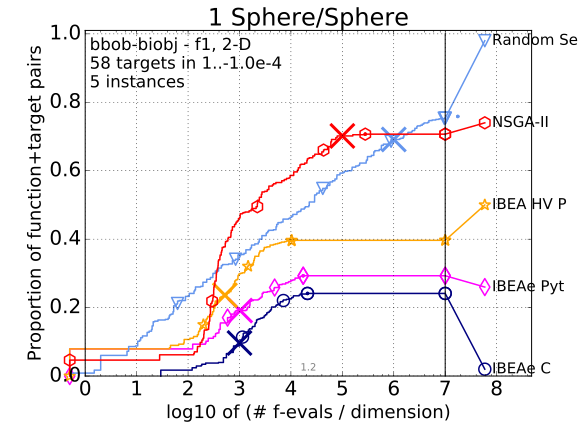
\includegraphics[width=0.2\textwidth]{pprldmany-single-functions/pprldmany_f001_02D}&
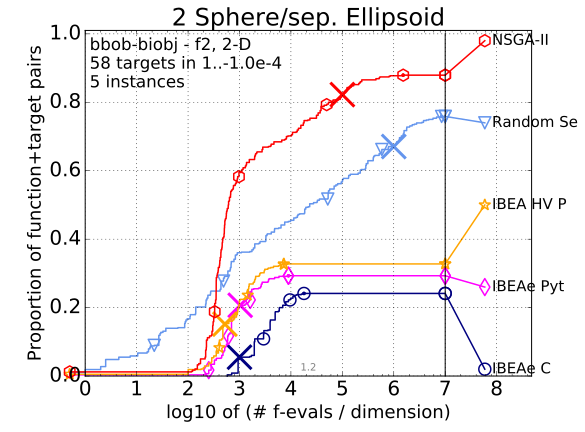
\includegraphics[width=0.2\textwidth]{pprldmany-single-functions/pprldmany_f002_02D}&
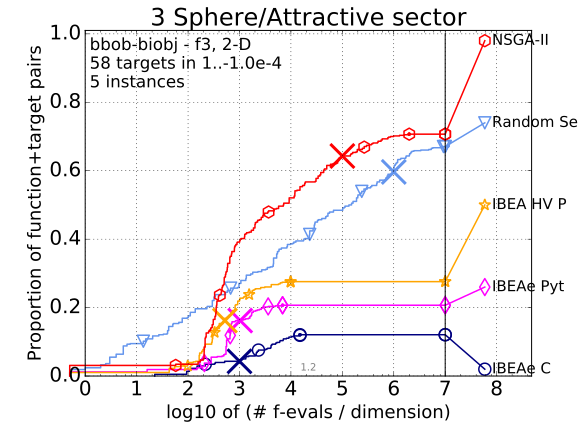
\includegraphics[width=0.2\textwidth]{pprldmany-single-functions/pprldmany_f003_02D}&
\includegraphics[width=0.2\textwidth]{pprldmany-single-functions/pprldmany_f004_02D}&
\includegraphics[width=0.2\textwidth]{pprldmany-single-functions/pprldmany_f005_02D}\\[-1.8ex]
\includegraphics[width=0.2\textwidth]{pprldmany-single-functions/pprldmany_f006_02D}&
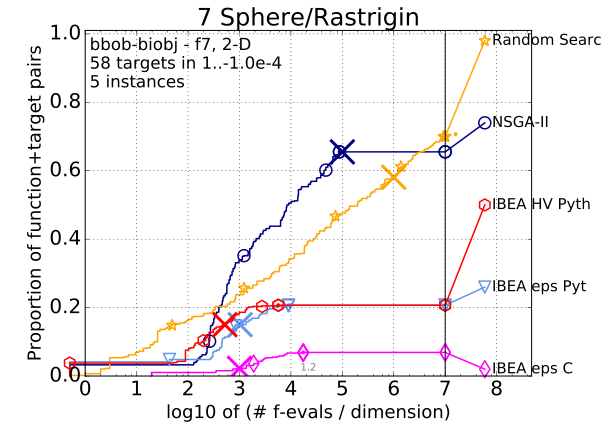
\includegraphics[width=0.2\textwidth]{pprldmany-single-functions/pprldmany_f007_02D}&
\includegraphics[width=0.2\textwidth]{pprldmany-single-functions/pprldmany_f008_02D}&
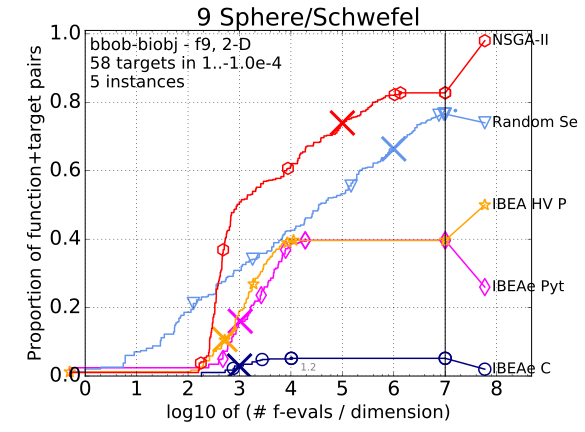
\includegraphics[width=0.2\textwidth]{pprldmany-single-functions/pprldmany_f009_02D}&
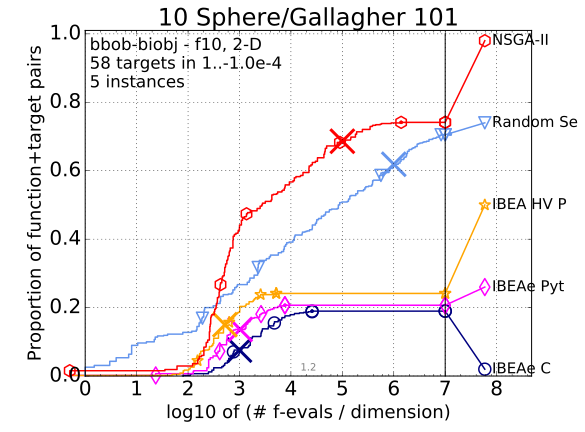
\includegraphics[width=0.2\textwidth]{pprldmany-single-functions/pprldmany_f010_02D}\\[-1.8ex]
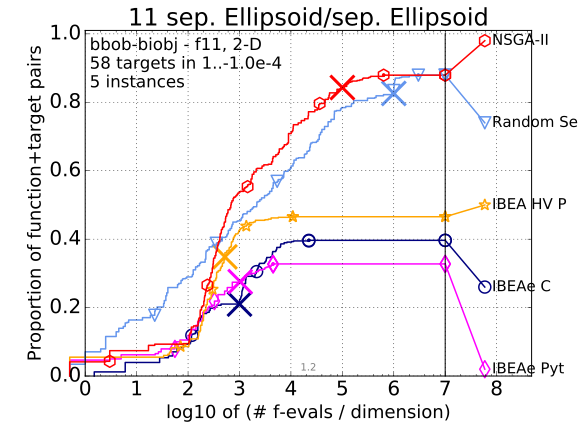
\includegraphics[width=0.2\textwidth]{pprldmany-single-functions/pprldmany_f011_02D}&
\includegraphics[width=0.2\textwidth]{pprldmany-single-functions/pprldmany_f012_02D}&
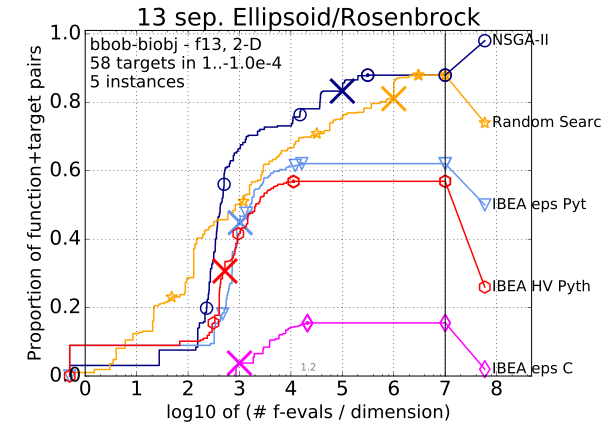
\includegraphics[width=0.2\textwidth]{pprldmany-single-functions/pprldmany_f013_02D}&
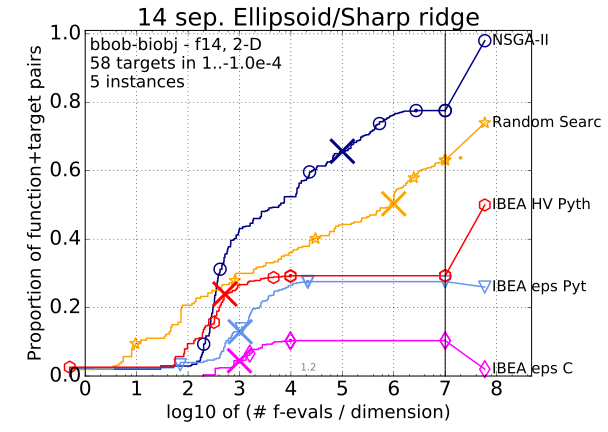
\includegraphics[width=0.2\textwidth]{pprldmany-single-functions/pprldmany_f014_02D}&
\includegraphics[width=0.2\textwidth]{pprldmany-single-functions/pprldmany_f015_02D}\\[-1.8ex]
\includegraphics[width=0.2\textwidth]{pprldmany-single-functions/pprldmany_f016_02D}&
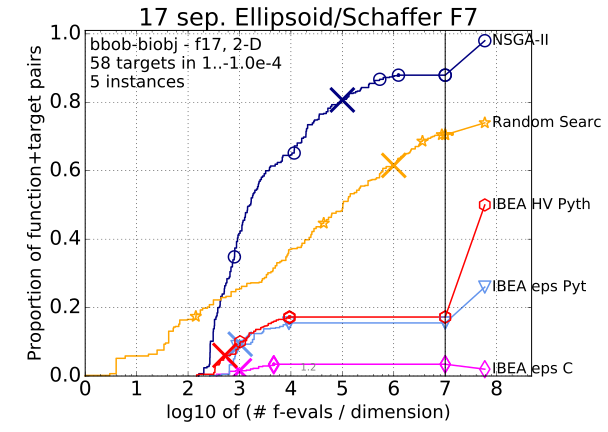
\includegraphics[width=0.2\textwidth]{pprldmany-single-functions/pprldmany_f017_02D}&
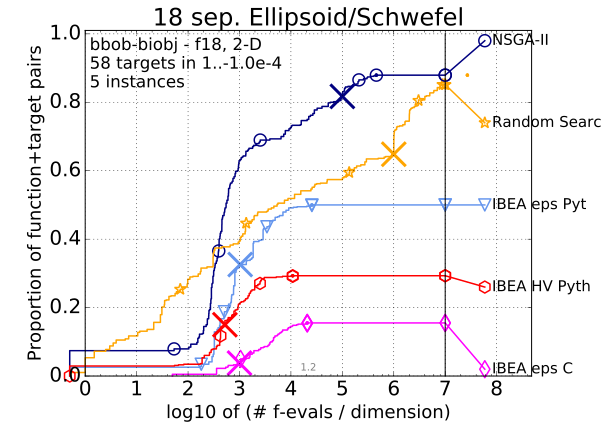
\includegraphics[width=0.2\textwidth]{pprldmany-single-functions/pprldmany_f018_02D}&
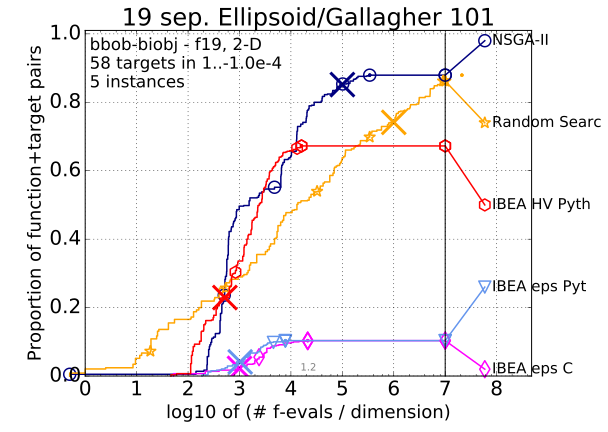
\includegraphics[width=0.2\textwidth]{pprldmany-single-functions/pprldmany_f019_02D}&
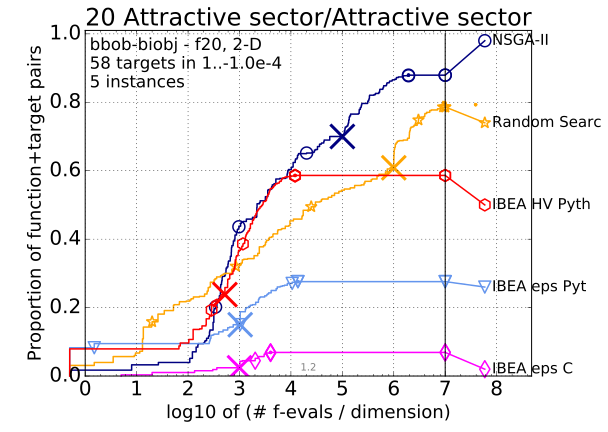
\includegraphics[width=0.2\textwidth]{pprldmany-single-functions/pprldmany_f020_02D}\\[-1.8ex]
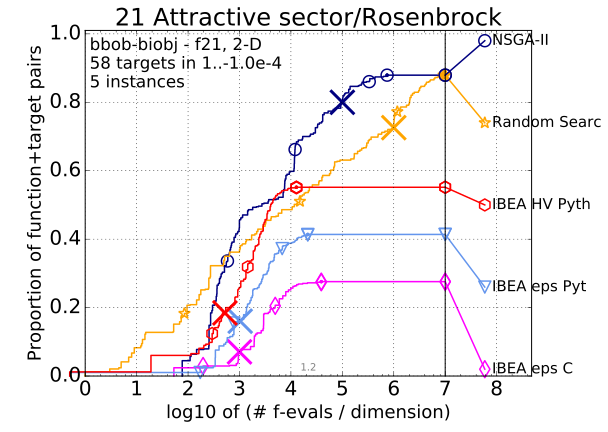
\includegraphics[width=0.2\textwidth]{pprldmany-single-functions/pprldmany_f021_02D}&
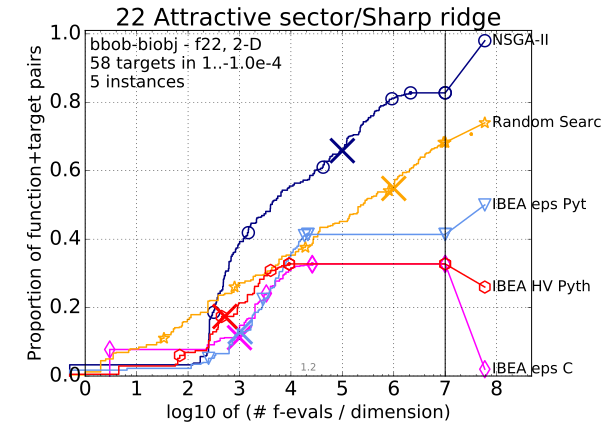
\includegraphics[width=0.2\textwidth]{pprldmany-single-functions/pprldmany_f022_02D}&
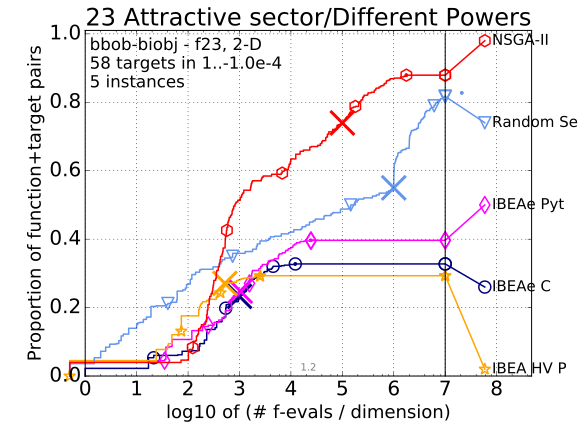
\includegraphics[width=0.2\textwidth]{pprldmany-single-functions/pprldmany_f023_02D}&
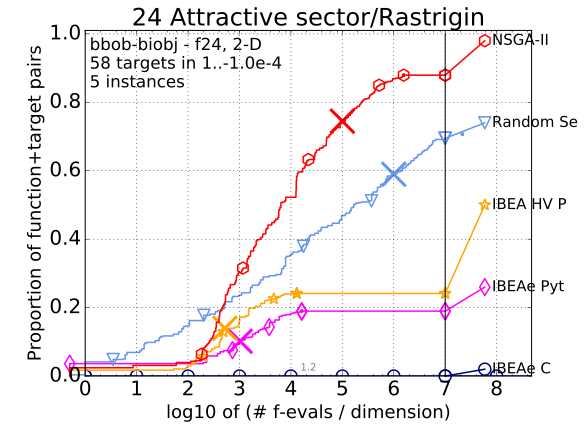
\includegraphics[width=0.2\textwidth]{pprldmany-single-functions/pprldmany_f024_02D}&
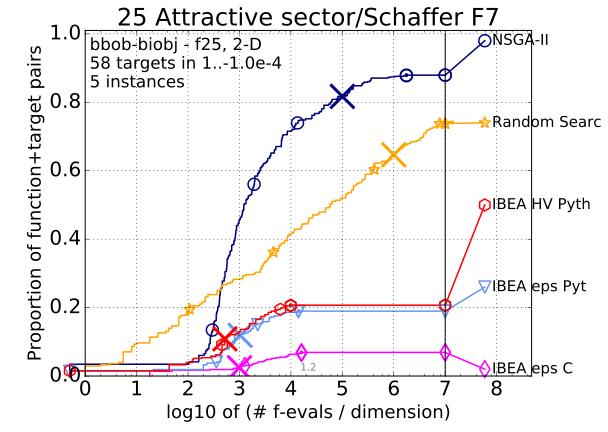
\includegraphics[width=0.2\textwidth]{pprldmany-single-functions/pprldmany_f025_02D}\\[-1.8ex]
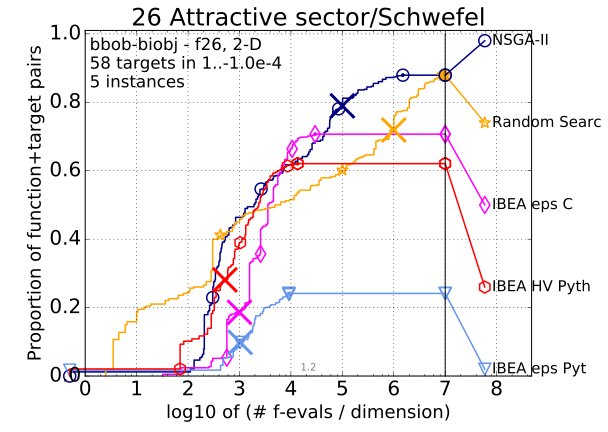
\includegraphics[width=0.2\textwidth]{pprldmany-single-functions/pprldmany_f026_02D}&
\includegraphics[width=0.2\textwidth]{pprldmany-single-functions/pprldmany_f027_02D}&
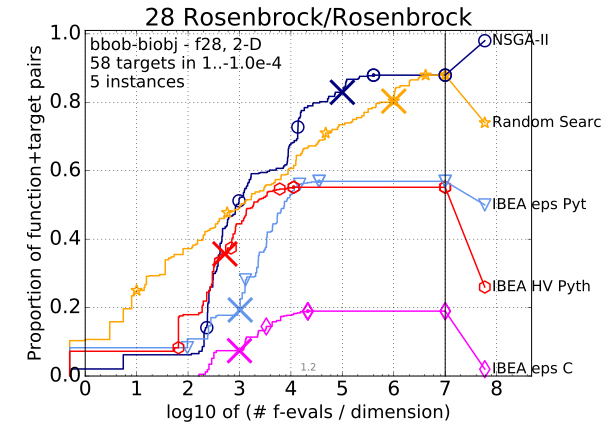
\includegraphics[width=0.2\textwidth]{pprldmany-single-functions/pprldmany_f028_02D}&
\includegraphics[width=0.2\textwidth]{pprldmany-single-functions/pprldmany_f029_02D}&
\includegraphics[width=0.2\textwidth]{pprldmany-single-functions/pprldmany_f030_02D}\\[-1.8ex]
\includegraphics[width=0.2\textwidth]{pprldmany-single-functions/pprldmany_f031_02D}&
\includegraphics[width=0.2\textwidth]{pprldmany-single-functions/pprldmany_f032_02D}&
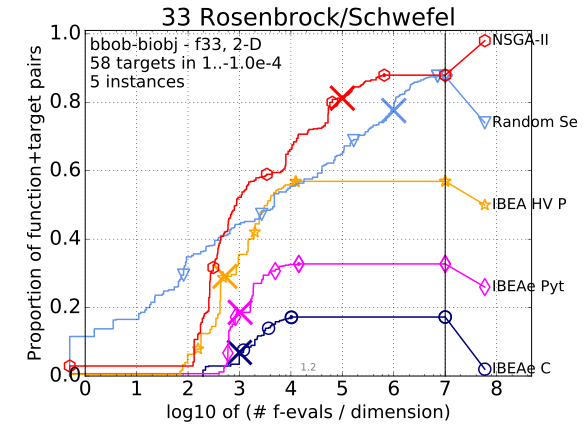
\includegraphics[width=0.2\textwidth]{pprldmany-single-functions/pprldmany_f033_02D}&
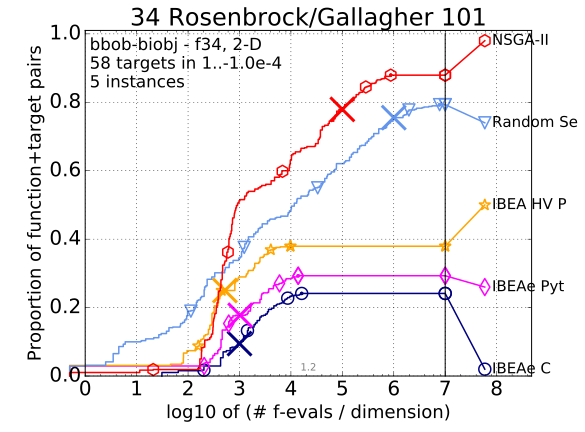
\includegraphics[width=0.2\textwidth]{pprldmany-single-functions/pprldmany_f034_02D}&
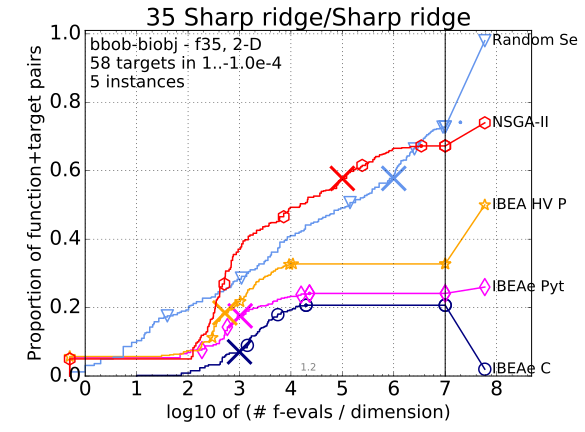
\includegraphics[width=0.2\textwidth]{pprldmany-single-functions/pprldmany_f035_02D}\\[-1.8ex]
\includegraphics[width=0.2\textwidth]{pprldmany-single-functions/pprldmany_f036_02D}&
\includegraphics[width=0.2\textwidth]{pprldmany-single-functions/pprldmany_f037_02D}&
\includegraphics[width=0.2\textwidth]{pprldmany-single-functions/pprldmany_f038_02D}&
\includegraphics[width=0.2\textwidth]{pprldmany-single-functions/pprldmany_f039_02D}&
\includegraphics[width=0.2\textwidth]{pprldmany-single-functions/pprldmany_f040_02D}\\[-1.8ex]

\end{tabular}
 \caption{\label{fig:ECDFsingleOne}
 Bootstrapped empirical cumulative distribution of the number of objective function evaluations divided by dimension (FEvals/DIM) for $58$ targets with target precision in $\{-10^{-4}, -10^{-4.2}, $ $-10^{-4.4}, -10^{-4.6}, -10^{-4.8}, -10^{-5}, 0, 10^{-5}, 10^{-4.9}, 10^{-4.8}, \dots, 10^{-0.1}, 10^0\}$ for each single function $f_{1}$ to $f_{40}$ in 10-D. 
}
\end{figure*}

\begin{figure*}
\centering
\begin{tabular}{@{\hspace*{-0.005\textwidth}}l@{\hspace*{-0.005\textwidth}}l@{\hspace*{-0.005\textwidth}}l@{\hspace*{-0.005\textwidth}}l@{\hspace*{-0.005\textwidth}}l@{\hspace*{-0.005\textwidth}}}
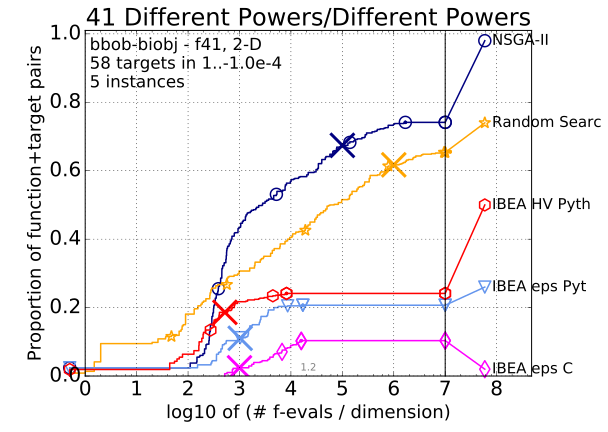
\includegraphics[width=0.2\textwidth]{pprldmany-single-functions/pprldmany_f041_02D}&
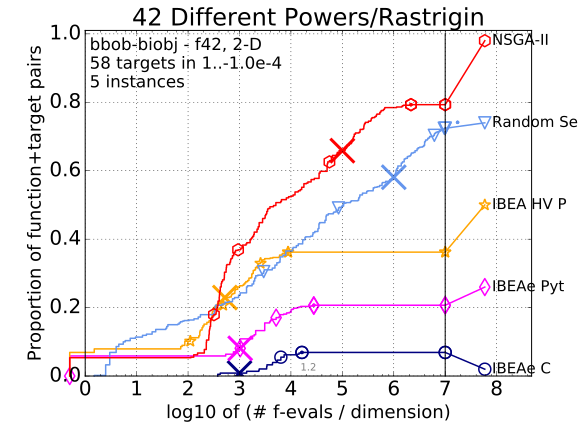
\includegraphics[width=0.2\textwidth]{pprldmany-single-functions/pprldmany_f042_02D}&
\includegraphics[width=0.2\textwidth]{pprldmany-single-functions/pprldmany_f043_02D}&
\includegraphics[width=0.2\textwidth]{pprldmany-single-functions/pprldmany_f044_02D}&
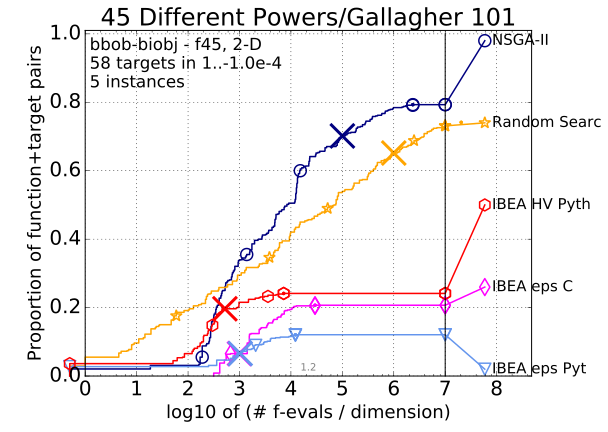
\includegraphics[width=0.2\textwidth]{pprldmany-single-functions/pprldmany_f045_02D}\\[-1.8ex]
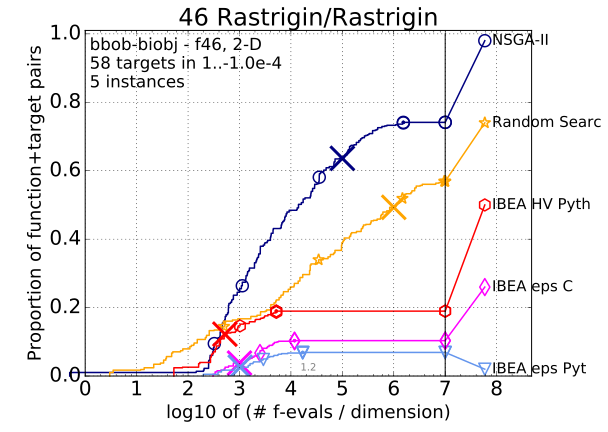
\includegraphics[width=0.2\textwidth]{pprldmany-single-functions/pprldmany_f046_02D}&
\includegraphics[width=0.2\textwidth]{pprldmany-single-functions/pprldmany_f047_02D}&
\includegraphics[width=0.2\textwidth]{pprldmany-single-functions/pprldmany_f048_02D}&
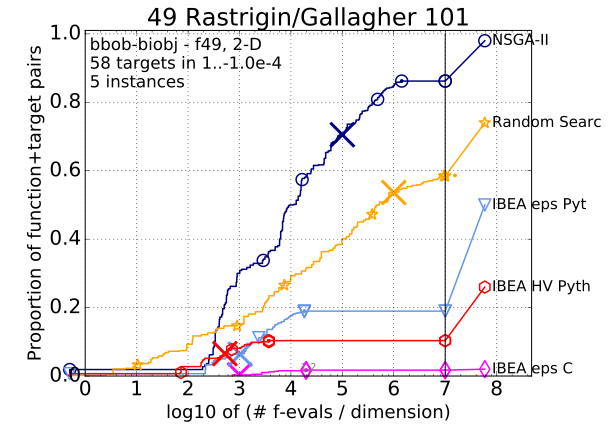
\includegraphics[width=0.2\textwidth]{pprldmany-single-functions/pprldmany_f049_02D}&
\includegraphics[width=0.2\textwidth]{pprldmany-single-functions/pprldmany_f040_02D}\\[-1.8ex]
\includegraphics[width=0.2\textwidth]{pprldmany-single-functions/pprldmany_f051_02D}&
\includegraphics[width=0.2\textwidth]{pprldmany-single-functions/pprldmany_f052_02D}&
\includegraphics[width=0.2\textwidth]{pprldmany-single-functions/pprldmany_f053_02D}&
\includegraphics[width=0.2\textwidth]{pprldmany-single-functions/pprldmany_f054_02D}&
\includegraphics[width=0.2\textwidth]{pprldmany-single-functions/pprldmany_f055_02D}\\[-1.8ex]
\end{tabular}
 \caption{\label{fig:ECDFsingleTwo}
 Bootstrapped empirical cumulative distribution of the number of objective function evaluations divided by dimension (FEvals/DIM) as in Fig.~\ref{fig:ECDFsingleOne} but for functions $f_{41}$ to $f_{55}$ in 10-D.
}
\end{figure*}




%%%%%%%%%%%%%%%%%%%%%%%%%%%%%%%%%%%%%%%%%%%%%%%%%%%%%%%%%%%%%%%%%%%%%%%%%%%%%%%
%%%%%%%%%%%%%%%%%%%%%%%%%%%%%%%%%%%%%%%%%%%%%%%%%%%%%%%%%%%%%%%%%%%%%%%%%%%%%%%

% Empirical cumulative distribution functions (ECDFs) per function group (5-D)

%%%%%%%%%%%%%%%%%%%%%%%%%%%%%%%%%%%%%%%%%%%%%%%%%%%%%%%%%%%%%%%%%%%%%%%%%%%%%%%

\begin{figure*}
\begin{tabular}{@{\hspace*{-0.009\textwidth}}c@{\hspace*{-0.014\textwidth}}c@{\hspace*{-0.016\textwidth}}c@{\hspace*{-0.02\textwidth}}c}
separable-separable & separable-moderate & separable-ill-cond. & separable-multimodal\\
\includegraphics[width=0.268\textwidth,trim=0 0 0 13mm, clip]{pprldmany_02D_1-separable_1-separable} &
\includegraphics[width=0.268\textwidth,trim=0 0 0 13mm, clip]{pprldmany_02D_1-separable_2-moderate} &
\includegraphics[width=0.268\textwidth,trim=0 0 0 13mm, clip]{pprldmany_02D_1-separable_3-ill-conditioned} &
\includegraphics[width=0.268\textwidth,trim=0 0 0 13mm, clip]{pprldmany_02D_1-separable_4-multi-modal}\\
separable-weakstructure & moderate-moderate & moderate-ill-cond. & moderate-multimodal\\
\includegraphics[width=0.268\textwidth,trim=0 0 0 13mm, clip]{pprldmany_02D_1-separable_5-weakly-structured} &
\includegraphics[width=0.268\textwidth,trim=0 0 0 13mm, clip]{pprldmany_02D_2-moderate_2-moderate} &
\includegraphics[width=0.268\textwidth,trim=0 0 0 13mm, clip]{pprldmany_02D_2-moderate_3-ill-conditioned} &
\includegraphics[width=0.268\textwidth,trim=0 0 0 13mm, clip]{pprldmany_02D_2-moderate_4-multi-modal}\\
moderate-weakstructure & ill-cond.-ill-cond. & ill-cond.-multimodal & ill-cond.-weakstructure\\
\includegraphics[width=0.268\textwidth,trim=0 0 0 13mm, clip]{pprldmany_02D_2-moderate_5-weakly-structured} &
\includegraphics[width=0.268\textwidth,trim=0 0 0 13mm, clip]{pprldmany_02D_3-ill-conditioned_3-ill-conditioned} &
\includegraphics[width=0.268\textwidth,trim=0 0 0 13mm, clip]{pprldmany_02D_3-ill-conditioned_4-multi-modal} &
\includegraphics[width=0.268\textwidth,trim=0 0 0 13mm, clip]{pprldmany_02D_3-ill-conditioned_5-weakly-structured} \\
multimodal-multimodal & multimodal-weakstructure & weakstructure-weakstructure & all 55 functions\\
\includegraphics[width=0.268\textwidth,trim=0 0 0 13mm, clip]{pprldmany_02D_4-multi-modal_4-multi-modal} &
\includegraphics[width=0.268\textwidth,trim=0 0 0 13mm, clip]{pprldmany_02D_4-multi-modal_5-weakly-structured} &
\includegraphics[width=0.268\textwidth,trim=0 0 0 13mm, clip]{pprldmany_02D_5-weakly-structured_5-weakly-structured} &
\includegraphics[width=0.268\textwidth,trim=0 0 0 13mm, clip]{pprldmany_02D_noiselessall}
\vspace*{-0.5ex}
\end{tabular}
 \caption{\label{fig:ECDFsGroupsFive}
 \bbobECDFslegend{4}
 }
\end{figure*}

%%%%%%%%%%%%%%%%%%%%%%%%%%%%%%%%%%%%%%%%%%%%%%%%%%%%%%%%%%%%%%%%%%%%%%%%%%%%%%%
%%%%%%%%%%%%%%%%%%%%%%%%%%%%%%%%%%%%%%%%%%%%%%%%%%%%%%%%%%%%%%%%%%%%%%%%%%%%%%%

% Empirical cumulative distribution functions (ECDFs) per function group (20-D)

%%%%%%%%%%%%%%%%%%%%%%%%%%%%%%%%%%%%%%%%%%%%%%%%%%%%%%%%%%%%%%%%%%%%%%%%%%%%%%%

%\begin{figure*}
%\begin{tabular}{@{\hspace*{-0.009\textwidth}}c@{\hspace*{-0.014\textwidth}}c@{\hspace*{-0.016\textwidth}}c@{\hspace*{-0.02\textwidth}}c}
%separable-separable & separable-moderate & separable-ill-cond. & separable-multimodal\\
%\includegraphics[width=0.268\textwidth,trim=0 0 0 13mm, clip]{pprldmany_20D_1-separable_1-separable} &
%\includegraphics[width=0.268\textwidth,trim=0 0 0 13mm, clip]{pprldmany_20D_1-separable_2-moderate} &
%\includegraphics[width=0.268\textwidth,trim=0 0 0 13mm, clip]{pprldmany_20D_1-separable_3-ill-conditioned} &
%\includegraphics[width=0.268\textwidth,trim=0 0 0 13mm, clip]{pprldmany_20D_1-separable_4-multi-modal}\\
%separable-weakstructure & moderate-moderate & moderate-ill-cond. & moderate-multimodal\\
%\includegraphics[width=0.268\textwidth,trim=0 0 0 13mm, clip]{pprldmany_20D_1-separable_5-weakly-structured} &
%\includegraphics[width=0.268\textwidth,trim=0 0 0 13mm, clip]{pprldmany_20D_2-moderate_2-moderate} &
%\includegraphics[width=0.268\textwidth,trim=0 0 0 13mm, clip]{pprldmany_20D_2-moderate_3-ill-conditioned} &
%\includegraphics[width=0.268\textwidth,trim=0 0 0 13mm, clip]{pprldmany_20D_2-moderate_4-multi-modal}\\
%moderate-weakstructure & ill-cond.-ill-cond. & ill-cond.-multimodal & ill-cond.-weakstructure\\
%\includegraphics[width=0.268\textwidth,trim=0 0 0 13mm, clip]{pprldmany_20D_2-moderate_5-weakly-structured} &
%\includegraphics[width=0.268\textwidth,trim=0 0 0 13mm, clip]{pprldmany_20D_3-ill-conditioned_3-ill-conditioned} &
%\includegraphics[width=0.268\textwidth,trim=0 0 0 13mm, clip]{pprldmany_20D_3-ill-conditioned_4-multi-modal} &
%\includegraphics[width=0.268\textwidth,trim=0 0 0 13mm, clip]{pprldmany_20D_3-ill-conditioned_5-weakly-structured} \\
%multimodal-multimodal & multimodal-weakstructure & weakstructure-weakstructure & all 55 functions\\
%\includegraphics[width=0.268\textwidth,trim=0 0 0 13mm, clip]{pprldmany_20D_4-multi-modal_4-multi-modal} &
%\includegraphics[width=0.268\textwidth,trim=0 0 0 13mm, clip]{pprldmany_20D_4-multi-modal_5-weakly-structured} &
%\includegraphics[width=0.268\textwidth,trim=0 0 0 13mm, clip]{pprldmany_20D_5-weakly-structured_5-weakly-structured} &
%\includegraphics[width=0.268\textwidth,trim=0 0 0 13mm, clip]{pprldmany_20D_noiselessall}
%\vspace*{-0.5ex}
%\end{tabular}
% \caption{\label{fig:ECDFsGroupsTwenty}
% \bbobECDFslegend{20}
% }
%\end{figure*}


\clearpage

%%%%%%%%%%%%%%%%%%%%%%%%%%%%%%%%%%%%%%%%%%%%%%%%%%%%%%%%%%%%%%%%%%%%%%%%%%%%%%%
%%%%%%%%%%%%%%%%%%%%%%%%%%%%%%%%%%%%%%%%%%%%%%%%%%%%%%%%%%%%%%%%%%%%%%%%%%%%%%%

% Average runtime (aRT in number of function evaluations)
% for functions $f_1$--$f_{55}$ of the bbob-biobj suite for dimension 5.

%%%%%%%%%%%%%%%%%%%%%%%%%%%%%%%%%%%%%%%%%%%%%%%%%%%%%%%%%%%%%%%%%%%%%%%%%%%%%%%
\begin{table*}\tiny
\centering
\mbox{\begin{minipage}[t]{0.32\textwidth}\tiny
\centering
\input{\bbobdatapath pptables_f001_02D} 

\input{\bbobdatapath pptables_f002_02D}

\input{\bbobdatapath pptables_f003_02D}

\input{\bbobdatapath pptables_f004_02D}

\input{\bbobdatapath pptables_f005_02D}

\input{\bbobdatapath pptables_f006_02D}

\input{\bbobdatapath pptables_f007_02D}

\input{\bbobdatapath pptables_f008_02D}

\input{\bbobdatapath pptables_f009_02D}

\input{\bbobdatapath pptables_f010_02D}

\input{\bbobdatapath pptables_f011_02D}

\input{\bbobdatapath pptables_f012_02D}

\input{\bbobdatapath pptables_f013_02D}

\input{\bbobdatapath pptables_f014_02D}

\input{\bbobdatapath pptables_f015_02D}

\input{\bbobdatapath pptables_f016_02D}

\input{\bbobdatapath pptables_f017_02D}

\input{\bbobdatapath pptables_f018_02D}

\input{\bbobdatapath pptables_f019_02D}

\end{minipage}
\hspace{0.002\textwidth}
\begin{minipage}[t]{0.32\textwidth}\tiny
\centering

\input{\bbobdatapath pptables_f020_02D}

\input{\bbobdatapath pptables_f021_02D}

\input{\bbobdatapath pptables_f022_02D}

\input{\bbobdatapath pptables_f023_02D}

\input{\bbobdatapath pptables_f024_02D}

\input{\bbobdatapath pptables_f025_02D}

\input{\bbobdatapath pptables_f026_02D}

\input{\bbobdatapath pptables_f027_02D}

\input{\bbobdatapath pptables_f028_02D}

\input{\bbobdatapath pptables_f029_02D}

\input{\bbobdatapath pptables_f030_02D}

\input{\bbobdatapath pptables_f031_02D}

\input{\bbobdatapath pptables_f032_02D}

\input{\bbobdatapath pptables_f033_02D}

\input{\bbobdatapath pptables_f034_02D}

\input{\bbobdatapath pptables_f035_02D}

\input{\bbobdatapath pptables_f036_02D}

\input{\bbobdatapath pptables_f037_02D}

\end{minipage}

\hspace{0.002\textwidth}
\begin{minipage}[t]{0.32\textwidth}\tiny
\centering

\input{\bbobdatapath pptables_f038_02D}

\input{\bbobdatapath pptables_f039_02D}

\input{\bbobdatapath pptables_f040_02D}

\input{\bbobdatapath pptables_f041_02D}

\input{\bbobdatapath pptables_f042_02D}

\input{\bbobdatapath pptables_f043_02D}

\input{\bbobdatapath pptables_f044_02D}

\input{\bbobdatapath pptables_f045_02D}

\input{\bbobdatapath pptables_f046_02D}

\input{\bbobdatapath pptables_f047_02D}

\input{\bbobdatapath pptables_f048_02D}

\input{\bbobdatapath pptables_f049_02D}

\input{\bbobdatapath pptables_f050_02D}

\input{\bbobdatapath pptables_f051_02D}

\input{\bbobdatapath pptables_f052_02D}

\input{\bbobdatapath pptables_f053_02D}

\input{\bbobdatapath pptables_f054_02D}

\input{\bbobdatapath pptables_f055_02D}

\end{minipage}}

 \caption{\label{tab:aRTs5}
 \bbobpptablesmanylegend{dimension $5$}{110} % Bonferroni correction: #dimensions * #functions
 }
\end{table*}
%sideways


%%%%%%%%%%%%%%%%%%%%%%%%%%%%%%%%%%%%%%%%%%%%%%%%%%%%%%%%%%%%%%%%%%%%%%%%%%%%%%%
%%%%%%%%%%%%%%%%%%%%%%%%%%%%%%%%%%%%%%%%%%%%%%%%%%%%%%%%%%%%%%%%%%%%%%%%%%%%%%%

% Average runtime (aRT in number of function evaluations)
% for functions $f_1$--$f_{55}$ of the bbob-biobj suite for dimension 20.

%%%%%%%%%%%%%%%%%%%%%%%%%%%%%%%%%%%%%%%%%%%%%%%%%%%%%%%%%%%%%%%%%%%%%%%%%%%%%%%
%\begin{table*}\tiny
%\centering
%\mbox{\begin{minipage}[t]{0.32\textwidth}\tiny
%\centering
%\input{\bbobdatapath pptables_f001_05D} 
%
%\input{\bbobdatapath pptables_f002_05D}
%
%\input{\bbobdatapath pptables_f003_05D}
%
%\input{\bbobdatapath pptables_f004_05D}
%
%\input{\bbobdatapath pptables_f005_05D}
%
%\input{\bbobdatapath pptables_f006_05D}
%
%\input{\bbobdatapath pptables_f007_05D}
%
%\input{\bbobdatapath pptables_f008_05D}
%
%\input{\bbobdatapath pptables_f009_05D}
%
%\input{\bbobdatapath pptables_f010_05D}
%
%\input{\bbobdatapath pptables_f011_05D}
%
%\input{\bbobdatapath pptables_f012_05D}
%
%\input{\bbobdatapath pptables_f013_05D}
%
%\input{\bbobdatapath pptables_f014_05D}
%
%\input{\bbobdatapath pptables_f015_05D}
%
%\input{\bbobdatapath pptables_f016_05D}
%
%\input{\bbobdatapath pptables_f017_05D}
%
%\input{\bbobdatapath pptables_f018_05D}
%
%\input{\bbobdatapath pptables_f019_05D}
%
%\end{minipage}
%\hspace{0.002\textwidth}
%\begin{minipage}[t]{0.32\textwidth}\tiny
%\centering
%
%\input{\bbobdatapath pptables_f020_05D}
%
%\input{\bbobdatapath pptables_f021_05D}
%
%\input{\bbobdatapath pptables_f022_05D}
%
%\input{\bbobdatapath pptables_f023_05D}
%
%\input{\bbobdatapath pptables_f024_05D}
%
%\input{\bbobdatapath pptables_f025_05D}
%
%\input{\bbobdatapath pptables_f026_05D}
%
%\input{\bbobdatapath pptables_f027_05D}
%
%\input{\bbobdatapath pptables_f028_05D}
%
%\input{\bbobdatapath pptables_f029_05D}
%
%\input{\bbobdatapath pptables_f030_05D}
%
%\input{\bbobdatapath pptables_f031_05D}
%
%\input{\bbobdatapath pptables_f032_05D}
%
%\input{\bbobdatapath pptables_f033_05D}
%
%\input{\bbobdatapath pptables_f034_05D}
%
%\input{\bbobdatapath pptables_f035_05D}
%
%\input{\bbobdatapath pptables_f036_05D}
%
%\input{\bbobdatapath pptables_f037_05D}
%
%\end{minipage}
%
%\hspace{0.002\textwidth}
%\begin{minipage}[t]{0.32\textwidth}\tiny
%\centering
%
%\input{\bbobdatapath pptables_f038_05D}
%
%\input{\bbobdatapath pptables_f039_05D}
%
%\input{\bbobdatapath pptables_f040_05D}
%
%\input{\bbobdatapath pptables_f041_05D}
%
%\input{\bbobdatapath pptables_f042_05D}
%
%\input{\bbobdatapath pptables_f043_05D}
%
%\input{\bbobdatapath pptables_f044_05D}
%
%\input{\bbobdatapath pptables_f045_05D}
%
%\input{\bbobdatapath pptables_f046_05D}
%
%\input{\bbobdatapath pptables_f047_05D}
%
%\input{\bbobdatapath pptables_f048_05D}
%
%\input{\bbobdatapath pptables_f049_05D}
%
%\input{\bbobdatapath pptables_f050_05D}
%
%\input{\bbobdatapath pptables_f051_05D}
%
%\input{\bbobdatapath pptables_f052_05D}
%
%\input{\bbobdatapath pptables_f053_05D}
%
%\input{\bbobdatapath pptables_f054_05D}
%
%\input{\bbobdatapath pptables_f055_05D}
%
%\end{minipage}}
%
% \caption{\label{tab:aRTs20}
% \bbobpptablesmanylegend{dimension $5$}{55} % Bonferroni correction: #dimensions * #functions
% }
%\end{table*}
%


%%%%%%%%%%%%%%%%%%%%%%%%%%%%%%%%%%%%%%%%%%%%%%%%%%%%%%%%%%%%%%%%%%%%%%%%%%%%%%%
% REFERENCES
%%%%%%%%%%%%%%%%%%%%%%%%%%%%%%%%%%%%%%%%%%%%%%%%%%%%%%%%%%%%%%%%%%%%%%%%%%%%%%%
% The following two commands are all you need in the
% initial runs of your .tex file to
% produce the bibliography for the citations in your paper.

\bibliographystyle{abbrv}
\bibliography{report.bib}
%\bibliographystyle{abbrv}
%\bibliography{bbob}  % bbob.bib is the name of the Bibliography in this case
% You must have a proper ".bib" file and remember to run:
% latex bibtex latex latex
% to resolve all references
% to create the ~.bbl file.  Insert that ~.bbl file into
% the .tex source file and comment out
% the command \texttt{{\char'134}thebibliography}.
%
% ACM needs 'a single self-contained file'!
%
\clearpage % otherwise the last figure might be missing

% Please uncomment for final version to fit paper to 8 pages.
\end{document}